% SOURCE: edit-harness/results/frame_a/cells/cell_*_real_MIX_{A,B,C}_*.json
% !TEX encoding = UTF-8 Unicode
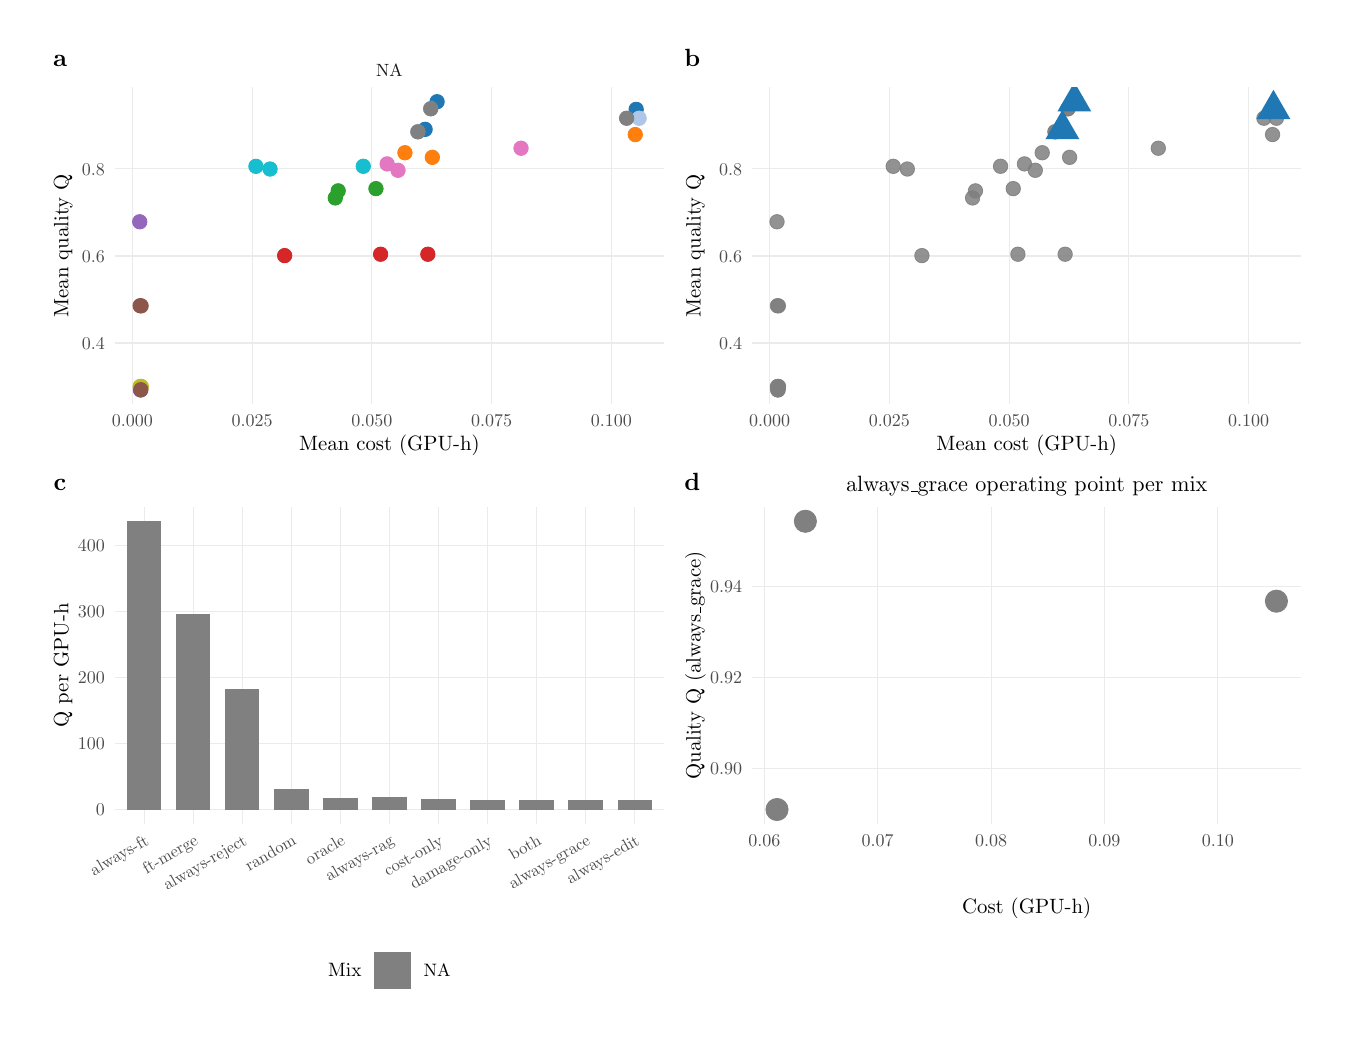
\begin{tikzpicture}[x=1pt,y=1pt]
\definecolor{fillColor}{RGB}{255,255,255}
\path[use as bounding box,fill=fillColor,fill opacity=0.00] (0,0) rectangle (469.75,361.35);
\begin{scope}
\path[clip] (  0.00,  0.00) rectangle (469.75,361.35);
\definecolor{drawColor}{RGB}{255,255,255}
\definecolor{fillColor}{RGB}{255,255,255}

\path[draw=drawColor,line width= 0.6pt,line join=round,line cap=round,fill=fillColor] (  0.00,  0.00) rectangle (469.75,361.35);
\end{scope}
\begin{scope}
\path[clip] (  5.50,203.26) rectangle (233.97,355.85);
\definecolor{fillColor}{RGB}{255,255,255}

\path[fill=fillColor] (  5.50,203.26) rectangle (233.97,355.85);
\end{scope}
\begin{scope}
\path[clip] (233.97,203.26) rectangle (464.25,355.85);
\definecolor{fillColor}{RGB}{255,255,255}

\path[fill=fillColor] (233.97,203.26) rectangle (464.25,355.85);
\end{scope}
\begin{scope}
\path[clip] (  5.50,  5.50) rectangle (233.97,203.26);
\definecolor{fillColor}{RGB}{255,255,255}

\path[fill=fillColor] (  5.50,  5.50) rectangle (233.97,203.26);
\end{scope}
\begin{scope}
\path[clip] (233.97,  5.50) rectangle (464.25,203.26);
\definecolor{fillColor}{RGB}{255,255,255}

\path[fill=fillColor] (233.97,  5.50) rectangle (464.25,203.26);
\end{scope}
\begin{scope}
\path[clip] ( 31.47,225.22) rectangle (229.97,339.80);
\definecolor{drawColor}{gray}{0.92}

\path[draw=drawColor,line width= 0.4pt,line join=round] ( 31.47,247.40) --
	(229.97,247.40);

\path[draw=drawColor,line width= 0.4pt,line join=round] ( 31.47,278.85) --
	(229.97,278.85);

\path[draw=drawColor,line width= 0.4pt,line join=round] ( 31.47,310.31) --
	(229.97,310.31);

\path[draw=drawColor,line width= 0.4pt,line join=round] ( 37.80,225.22) --
	( 37.80,339.80);

\path[draw=drawColor,line width= 0.4pt,line join=round] ( 81.08,225.22) --
	( 81.08,339.80);

\path[draw=drawColor,line width= 0.4pt,line join=round] (124.37,225.22) --
	(124.37,339.80);

\path[draw=drawColor,line width= 0.4pt,line join=round] (167.65,225.22) --
	(167.65,339.80);

\path[draw=drawColor,line width= 0.4pt,line join=round] (210.93,225.22) --
	(210.93,339.80);
\definecolor{drawColor}{RGB}{255,127,14}
\definecolor{fillColor}{RGB}{255,127,14}

\path[draw=drawColor,line width= 0.3pt,line join=round,line cap=round,fill=fillColor] (146.22,314.49) circle (  2.61);
\definecolor{drawColor}{RGB}{148,103,189}
\definecolor{fillColor}{RGB}{148,103,189}

\path[draw=drawColor,line width= 0.3pt,line join=round,line cap=round,fill=fillColor] ( 40.49,291.21) circle (  2.61);
\definecolor{drawColor}{RGB}{31,119,180}
\definecolor{fillColor}{RGB}{31,119,180}

\path[draw=drawColor,line width= 0.3pt,line join=round,line cap=round,fill=fillColor] (147.94,334.59) circle (  2.61);
\definecolor{drawColor}{RGB}{214,39,40}
\definecolor{fillColor}{RGB}{214,39,40}

\path[draw=drawColor,line width= 0.3pt,line join=round,line cap=round,fill=fillColor] (127.53,279.48) circle (  2.61);
\definecolor{drawColor}{RGB}{188,189,34}
\definecolor{fillColor}{RGB}{188,189,34}

\path[draw=drawColor,line width= 0.3pt,line join=round,line cap=round,fill=fillColor] ( 40.64,231.67) circle (  2.61);
\definecolor{drawColor}{RGB}{174,199,232}
\definecolor{fillColor}{RGB}{174,199,232}

\path[draw=drawColor,line width= 0.3pt,line join=round,line cap=round,fill=fillColor] (145.57,332.05) circle (  2.61);
\definecolor{drawColor}{RGB}{227,119,194}
\definecolor{fillColor}{RGB}{227,119,194}

\path[draw=drawColor,line width= 0.3pt,line join=round,line cap=round,fill=fillColor] (133.82,309.81) circle (  2.61);
\definecolor{drawColor}{gray}{0.50}
\definecolor{fillColor}{gray}{0.50}

\path[draw=drawColor,line width= 0.3pt,line join=round,line cap=round,fill=fillColor] (145.67,332.05) circle (  2.61);
\definecolor{drawColor}{RGB}{140,86,75}
\definecolor{fillColor}{RGB}{140,86,75}

\path[draw=drawColor,line width= 0.3pt,line join=round,line cap=round,fill=fillColor] ( 40.64,260.87) circle (  2.61);
\definecolor{drawColor}{RGB}{44,160,44}
\definecolor{fillColor}{RGB}{44,160,44}

\path[draw=drawColor,line width= 0.3pt,line join=round,line cap=round,fill=fillColor] (112.20,302.38) circle (  2.61);
\definecolor{drawColor}{RGB}{23,190,207}
\definecolor{fillColor}{RGB}{23,190,207}

\path[draw=drawColor,line width= 0.3pt,line join=round,line cap=round,fill=fillColor] ( 82.48,311.24) circle (  2.61);
\definecolor{drawColor}{RGB}{255,127,14}
\definecolor{fillColor}{RGB}{255,127,14}

\path[draw=drawColor,line width= 0.3pt,line join=round,line cap=round,fill=fillColor] (136.32,316.16) circle (  2.61);
\definecolor{drawColor}{RGB}{148,103,189}
\definecolor{fillColor}{RGB}{148,103,189}

\path[draw=drawColor,line width= 0.3pt,line join=round,line cap=round,fill=fillColor] ( 40.81,230.43) circle (  2.61);
\definecolor{drawColor}{RGB}{31,119,180}
\definecolor{fillColor}{RGB}{31,119,180}

\path[draw=drawColor,line width= 0.3pt,line join=round,line cap=round,fill=fillColor] (143.61,324.61) circle (  2.61);
\definecolor{drawColor}{RGB}{214,39,40}
\definecolor{fillColor}{RGB}{214,39,40}

\path[draw=drawColor,line width= 0.3pt,line join=round,line cap=round,fill=fillColor] (144.60,279.48) circle (  2.61);
\definecolor{drawColor}{RGB}{188,189,34}
\definecolor{fillColor}{RGB}{188,189,34}

\path[draw=drawColor,line width= 0.3pt,line join=round,line cap=round,fill=fillColor] ( 41.04,231.67) circle (  2.61);
\definecolor{drawColor}{RGB}{174,199,232}
\definecolor{fillColor}{RGB}{174,199,232}

\path[draw=drawColor,line width= 0.3pt,line join=round,line cap=round,fill=fillColor] (140.89,323.72) circle (  2.61);
\definecolor{drawColor}{RGB}{227,119,194}
\definecolor{fillColor}{RGB}{227,119,194}

\path[draw=drawColor,line width= 0.3pt,line join=round,line cap=round,fill=fillColor] (129.90,312.12) circle (  2.61);
\definecolor{drawColor}{gray}{0.50}
\definecolor{fillColor}{gray}{0.50}

\path[draw=drawColor,line width= 0.3pt,line join=round,line cap=round,fill=fillColor] (141.04,323.72) circle (  2.61);
\definecolor{drawColor}{RGB}{140,86,75}
\definecolor{fillColor}{RGB}{140,86,75}

\path[draw=drawColor,line width= 0.3pt,line join=round,line cap=round,fill=fillColor] ( 40.99,260.82) circle (  2.61);
\definecolor{drawColor}{RGB}{44,160,44}
\definecolor{fillColor}{RGB}{44,160,44}

\path[draw=drawColor,line width= 0.3pt,line join=round,line cap=round,fill=fillColor] (111.16,299.82) circle (  2.61);
\definecolor{drawColor}{RGB}{23,190,207}
\definecolor{fillColor}{RGB}{23,190,207}

\path[draw=drawColor,line width= 0.3pt,line join=round,line cap=round,fill=fillColor] ( 87.58,310.27) circle (  2.61);
\definecolor{drawColor}{RGB}{255,127,14}
\definecolor{fillColor}{RGB}{255,127,14}

\path[draw=drawColor,line width= 0.3pt,line join=round,line cap=round,fill=fillColor] (219.55,322.72) circle (  2.61);
\definecolor{drawColor}{RGB}{148,103,189}
\definecolor{fillColor}{RGB}{148,103,189}

\path[draw=drawColor,line width= 0.3pt,line join=round,line cap=round,fill=fillColor] ( 40.74,230.52) circle (  2.61);
\definecolor{drawColor}{RGB}{31,119,180}
\definecolor{fillColor}{RGB}{31,119,180}

\path[draw=drawColor,line width= 0.3pt,line join=round,line cap=round,fill=fillColor] (219.88,331.82) circle (  2.61);
\definecolor{drawColor}{RGB}{214,39,40}
\definecolor{fillColor}{RGB}{214,39,40}

\path[draw=drawColor,line width= 0.3pt,line join=round,line cap=round,fill=fillColor] ( 92.85,278.98) circle (  2.61);
\definecolor{drawColor}{RGB}{188,189,34}
\definecolor{fillColor}{RGB}{188,189,34}

\path[draw=drawColor,line width= 0.3pt,line join=round,line cap=round,fill=fillColor] ( 40.88,231.67) circle (  2.61);
\definecolor{drawColor}{RGB}{174,199,232}
\definecolor{fillColor}{RGB}{174,199,232}

\path[draw=drawColor,line width= 0.3pt,line join=round,line cap=round,fill=fillColor] (220.95,328.62) circle (  2.61);
\definecolor{drawColor}{RGB}{227,119,194}
\definecolor{fillColor}{RGB}{227,119,194}

\path[draw=drawColor,line width= 0.3pt,line join=round,line cap=round,fill=fillColor] (178.27,317.78) circle (  2.61);
\definecolor{drawColor}{gray}{0.50}
\definecolor{fillColor}{gray}{0.50}

\path[draw=drawColor,line width= 0.3pt,line join=round,line cap=round,fill=fillColor] (216.43,328.62) circle (  2.61);
\definecolor{drawColor}{RGB}{140,86,75}
\definecolor{fillColor}{RGB}{140,86,75}

\path[draw=drawColor,line width= 0.3pt,line join=round,line cap=round,fill=fillColor] ( 40.88,230.52) circle (  2.61);
\definecolor{drawColor}{RGB}{44,160,44}
\definecolor{fillColor}{RGB}{44,160,44}

\path[draw=drawColor,line width= 0.3pt,line join=round,line cap=round,fill=fillColor] (125.85,303.18) circle (  2.61);
\definecolor{drawColor}{RGB}{23,190,207}
\definecolor{fillColor}{RGB}{23,190,207}

\path[draw=drawColor,line width= 0.3pt,line join=round,line cap=round,fill=fillColor] (121.27,311.26) circle (  2.61);
\end{scope}
\begin{scope}
\path[clip] ( 31.47,339.80) rectangle (229.97,351.85);
\definecolor{drawColor}{gray}{0.10}

\node[text=drawColor,anchor=base,inner sep=0pt, outer sep=0pt, scale=  0.64] at (130.72,343.62) {NA};
\end{scope}
\begin{scope}
\path[clip] (  0.00,  0.00) rectangle (469.75,361.35);
\definecolor{drawColor}{gray}{0.30}

\node[text=drawColor,anchor=base,inner sep=0pt, outer sep=0pt, scale=  0.65] at ( 37.80,217.15) {0.000};

\node[text=drawColor,anchor=base,inner sep=0pt, outer sep=0pt, scale=  0.65] at ( 81.08,217.15) {0.025};

\node[text=drawColor,anchor=base,inner sep=0pt, outer sep=0pt, scale=  0.65] at (124.37,217.15) {0.050};

\node[text=drawColor,anchor=base,inner sep=0pt, outer sep=0pt, scale=  0.65] at (167.65,217.15) {0.075};

\node[text=drawColor,anchor=base,inner sep=0pt, outer sep=0pt, scale=  0.65] at (210.93,217.15) {0.100};
\end{scope}
\begin{scope}
\path[clip] (  0.00,  0.00) rectangle (469.75,361.35);
\definecolor{drawColor}{gray}{0.30}

\node[text=drawColor,anchor=base east,inner sep=0pt, outer sep=0pt, scale=  0.65] at ( 27.87,245.16) {0.4};

\node[text=drawColor,anchor=base east,inner sep=0pt, outer sep=0pt, scale=  0.65] at ( 27.87,276.62) {0.6};

\node[text=drawColor,anchor=base east,inner sep=0pt, outer sep=0pt, scale=  0.65] at ( 27.87,308.07) {0.8};
\end{scope}
\begin{scope}
\path[clip] (  0.00,  0.00) rectangle (469.75,361.35);
\definecolor{drawColor}{RGB}{0,0,0}

\node[text=drawColor,anchor=base,inner sep=0pt, outer sep=0pt, scale=  0.75] at (130.72,208.72) {Mean cost (GPU-h)};
\end{scope}
\begin{scope}
\path[clip] (  0.00,  0.00) rectangle (469.75,361.35);
\definecolor{drawColor}{RGB}{0,0,0}

\node[text=drawColor,rotate= 90.00,anchor=base,inner sep=0pt, outer sep=0pt, scale=  0.75] at ( 14.67,282.51) {Mean quality Q};
\end{scope}
\begin{scope}
\path[clip] (  0.00,  0.00) rectangle (469.75,361.35);
\definecolor{drawColor}{RGB}{0,0,0}

\node[text=drawColor,anchor=base,inner sep=0pt, outer sep=0pt, scale=  0.90] at ( 11.70,347.30) {\bfseries a};
\end{scope}
\begin{scope}
\path[clip] (261.75,225.22) rectangle (460.26,339.80);
\definecolor{drawColor}{gray}{0.92}

\path[draw=drawColor,line width= 0.4pt,line join=round] (261.75,247.40) --
	(460.26,247.40);

\path[draw=drawColor,line width= 0.4pt,line join=round] (261.75,278.85) --
	(460.26,278.85);

\path[draw=drawColor,line width= 0.4pt,line join=round] (261.75,310.31) --
	(460.26,310.31);

\path[draw=drawColor,line width= 0.4pt,line join=round] (268.08,225.22) --
	(268.08,339.80);

\path[draw=drawColor,line width= 0.4pt,line join=round] (311.36,225.22) --
	(311.36,339.80);

\path[draw=drawColor,line width= 0.4pt,line join=round] (354.65,225.22) --
	(354.65,339.80);

\path[draw=drawColor,line width= 0.4pt,line join=round] (397.93,225.22) --
	(397.93,339.80);

\path[draw=drawColor,line width= 0.4pt,line join=round] (441.21,225.22) --
	(441.21,339.80);
\definecolor{drawColor}{RGB}{127,127,127}
\definecolor{fillColor}{RGB}{127,127,127}

\path[draw=drawColor,draw opacity=0.85,line width= 0.3pt,line join=round,line cap=round,fill=fillColor,fill opacity=0.85] (376.50,314.49) circle (  2.61);

\path[draw=drawColor,draw opacity=0.85,line width= 0.3pt,line join=round,line cap=round,fill=fillColor,fill opacity=0.85] (270.77,291.21) circle (  2.61);

\path[draw=drawColor,draw opacity=0.85,line width= 0.3pt,line join=round,line cap=round,fill=fillColor,fill opacity=0.85] (378.22,334.59) circle (  2.61);

\path[draw=drawColor,draw opacity=0.85,line width= 0.3pt,line join=round,line cap=round,fill=fillColor,fill opacity=0.85] (357.81,279.48) circle (  2.61);

\path[draw=drawColor,draw opacity=0.85,line width= 0.3pt,line join=round,line cap=round,fill=fillColor,fill opacity=0.85] (270.92,231.67) circle (  2.61);

\path[draw=drawColor,draw opacity=0.85,line width= 0.3pt,line join=round,line cap=round,fill=fillColor,fill opacity=0.85] (375.85,332.05) circle (  2.61);

\path[draw=drawColor,draw opacity=0.85,line width= 0.3pt,line join=round,line cap=round,fill=fillColor,fill opacity=0.85] (364.10,309.81) circle (  2.61);

\path[draw=drawColor,draw opacity=0.85,line width= 0.3pt,line join=round,line cap=round,fill=fillColor,fill opacity=0.85] (375.95,332.05) circle (  2.61);

\path[draw=drawColor,draw opacity=0.85,line width= 0.3pt,line join=round,line cap=round,fill=fillColor,fill opacity=0.85] (270.92,260.87) circle (  2.61);

\path[draw=drawColor,draw opacity=0.85,line width= 0.3pt,line join=round,line cap=round,fill=fillColor,fill opacity=0.85] (342.48,302.38) circle (  2.61);

\path[draw=drawColor,draw opacity=0.85,line width= 0.3pt,line join=round,line cap=round,fill=fillColor,fill opacity=0.85] (312.76,311.24) circle (  2.61);

\path[draw=drawColor,draw opacity=0.85,line width= 0.3pt,line join=round,line cap=round,fill=fillColor,fill opacity=0.85] (366.60,316.16) circle (  2.61);

\path[draw=drawColor,draw opacity=0.85,line width= 0.3pt,line join=round,line cap=round,fill=fillColor,fill opacity=0.85] (271.09,230.43) circle (  2.61);

\path[draw=drawColor,draw opacity=0.85,line width= 0.3pt,line join=round,line cap=round,fill=fillColor,fill opacity=0.85] (373.89,324.61) circle (  2.61);

\path[draw=drawColor,draw opacity=0.85,line width= 0.3pt,line join=round,line cap=round,fill=fillColor,fill opacity=0.85] (374.88,279.48) circle (  2.61);

\path[draw=drawColor,draw opacity=0.85,line width= 0.3pt,line join=round,line cap=round,fill=fillColor,fill opacity=0.85] (271.32,231.67) circle (  2.61);

\path[draw=drawColor,draw opacity=0.85,line width= 0.3pt,line join=round,line cap=round,fill=fillColor,fill opacity=0.85] (371.17,323.72) circle (  2.61);

\path[draw=drawColor,draw opacity=0.85,line width= 0.3pt,line join=round,line cap=round,fill=fillColor,fill opacity=0.85] (360.18,312.12) circle (  2.61);

\path[draw=drawColor,draw opacity=0.85,line width= 0.3pt,line join=round,line cap=round,fill=fillColor,fill opacity=0.85] (371.32,323.72) circle (  2.61);

\path[draw=drawColor,draw opacity=0.85,line width= 0.3pt,line join=round,line cap=round,fill=fillColor,fill opacity=0.85] (271.27,260.82) circle (  2.61);

\path[draw=drawColor,draw opacity=0.85,line width= 0.3pt,line join=round,line cap=round,fill=fillColor,fill opacity=0.85] (341.44,299.82) circle (  2.61);

\path[draw=drawColor,draw opacity=0.85,line width= 0.3pt,line join=round,line cap=round,fill=fillColor,fill opacity=0.85] (317.86,310.27) circle (  2.61);

\path[draw=drawColor,draw opacity=0.85,line width= 0.3pt,line join=round,line cap=round,fill=fillColor,fill opacity=0.85] (449.83,322.72) circle (  2.61);

\path[draw=drawColor,draw opacity=0.85,line width= 0.3pt,line join=round,line cap=round,fill=fillColor,fill opacity=0.85] (271.02,230.52) circle (  2.61);

\path[draw=drawColor,draw opacity=0.85,line width= 0.3pt,line join=round,line cap=round,fill=fillColor,fill opacity=0.85] (450.16,331.82) circle (  2.61);

\path[draw=drawColor,draw opacity=0.85,line width= 0.3pt,line join=round,line cap=round,fill=fillColor,fill opacity=0.85] (323.13,278.98) circle (  2.61);

\path[draw=drawColor,draw opacity=0.85,line width= 0.3pt,line join=round,line cap=round,fill=fillColor,fill opacity=0.85] (271.16,231.67) circle (  2.61);

\path[draw=drawColor,draw opacity=0.85,line width= 0.3pt,line join=round,line cap=round,fill=fillColor,fill opacity=0.85] (451.23,328.62) circle (  2.61);

\path[draw=drawColor,draw opacity=0.85,line width= 0.3pt,line join=round,line cap=round,fill=fillColor,fill opacity=0.85] (408.55,317.78) circle (  2.61);

\path[draw=drawColor,draw opacity=0.85,line width= 0.3pt,line join=round,line cap=round,fill=fillColor,fill opacity=0.85] (446.71,328.62) circle (  2.61);

\path[draw=drawColor,draw opacity=0.85,line width= 0.3pt,line join=round,line cap=round,fill=fillColor,fill opacity=0.85] (271.16,230.52) circle (  2.61);

\path[draw=drawColor,draw opacity=0.85,line width= 0.3pt,line join=round,line cap=round,fill=fillColor,fill opacity=0.85] (356.13,303.18) circle (  2.61);

\path[draw=drawColor,draw opacity=0.85,line width= 0.3pt,line join=round,line cap=round,fill=fillColor,fill opacity=0.85] (351.55,311.26) circle (  2.61);
\definecolor{fillColor}{RGB}{31,119,180}

\path[fill=fillColor] (378.22,341.65) --
	(384.34,331.06) --
	(372.10,331.06) --
	cycle;

\path[fill=fillColor] (373.89,331.67) --
	(380.01,321.07) --
	(367.77,321.07) --
	cycle;

\path[fill=fillColor] (450.16,338.89) --
	(456.28,328.29) --
	(444.05,328.29) --
	cycle;
\end{scope}
\begin{scope}
\path[clip] (  0.00,  0.00) rectangle (469.75,361.35);
\definecolor{drawColor}{gray}{0.30}

\node[text=drawColor,anchor=base east,inner sep=0pt, outer sep=0pt, scale=  0.65] at (258.15,245.16) {0.4};

\node[text=drawColor,anchor=base east,inner sep=0pt, outer sep=0pt, scale=  0.65] at (258.15,276.62) {0.6};

\node[text=drawColor,anchor=base east,inner sep=0pt, outer sep=0pt, scale=  0.65] at (258.15,308.07) {0.8};
\end{scope}
\begin{scope}
\path[clip] (  0.00,  0.00) rectangle (469.75,361.35);
\definecolor{drawColor}{gray}{0.30}

\node[text=drawColor,anchor=base,inner sep=0pt, outer sep=0pt, scale=  0.65] at (268.08,217.15) {0.000};

\node[text=drawColor,anchor=base,inner sep=0pt, outer sep=0pt, scale=  0.65] at (311.36,217.15) {0.025};

\node[text=drawColor,anchor=base,inner sep=0pt, outer sep=0pt, scale=  0.65] at (354.65,217.15) {0.050};

\node[text=drawColor,anchor=base,inner sep=0pt, outer sep=0pt, scale=  0.65] at (397.93,217.15) {0.075};

\node[text=drawColor,anchor=base,inner sep=0pt, outer sep=0pt, scale=  0.65] at (441.21,217.15) {0.100};
\end{scope}
\begin{scope}
\path[clip] (  0.00,  0.00) rectangle (469.75,361.35);
\definecolor{drawColor}{RGB}{0,0,0}

\node[text=drawColor,anchor=base,inner sep=0pt, outer sep=0pt, scale=  0.75] at (361.00,208.72) {Mean cost (GPU-h)};
\end{scope}
\begin{scope}
\path[clip] (  0.00,  0.00) rectangle (469.75,361.35);
\definecolor{drawColor}{RGB}{0,0,0}

\node[text=drawColor,rotate= 90.00,anchor=base,inner sep=0pt, outer sep=0pt, scale=  0.75] at (243.14,282.51) {Mean quality Q};
\end{scope}
\begin{scope}
\path[clip] (  0.00,  0.00) rectangle (469.75,361.35);
\definecolor{drawColor}{RGB}{0,0,0}

\node[text=drawColor,anchor=base,inner sep=0pt, outer sep=0pt, scale=  0.90] at (240.20,347.30) {\bfseries b};
\end{scope}
\begin{scope}
\path[clip] ( 31.47, 73.62) rectangle (229.97,188.20);
\definecolor{drawColor}{gray}{0.92}

\path[draw=drawColor,line width= 0.4pt,line join=round] ( 31.47, 78.83) --
	(229.97, 78.83);

\path[draw=drawColor,line width= 0.4pt,line join=round] ( 31.47,102.72) --
	(229.97,102.72);

\path[draw=drawColor,line width= 0.4pt,line join=round] ( 31.47,126.60) --
	(229.97,126.60);

\path[draw=drawColor,line width= 0.4pt,line join=round] ( 31.47,150.49) --
	(229.97,150.49);

\path[draw=drawColor,line width= 0.4pt,line join=round] ( 31.47,174.38) --
	(229.97,174.38);

\path[draw=drawColor,line width= 0.4pt,line join=round] ( 42.11, 73.62) --
	( 42.11,188.20);

\path[draw=drawColor,line width= 0.4pt,line join=round] ( 59.83, 73.62) --
	( 59.83,188.20);

\path[draw=drawColor,line width= 0.4pt,line join=round] ( 77.55, 73.62) --
	( 77.55,188.20);

\path[draw=drawColor,line width= 0.4pt,line join=round] ( 95.28, 73.62) --
	( 95.28,188.20);

\path[draw=drawColor,line width= 0.4pt,line join=round] (113.00, 73.62) --
	(113.00,188.20);

\path[draw=drawColor,line width= 0.4pt,line join=round] (130.72, 73.62) --
	(130.72,188.20);

\path[draw=drawColor,line width= 0.4pt,line join=round] (148.45, 73.62) --
	(148.45,188.20);

\path[draw=drawColor,line width= 0.4pt,line join=round] (166.17, 73.62) --
	(166.17,188.20);

\path[draw=drawColor,line width= 0.4pt,line join=round] (183.89, 73.62) --
	(183.89,188.20);

\path[draw=drawColor,line width= 0.4pt,line join=round] (201.62, 73.62) --
	(201.62,188.20);

\path[draw=drawColor,line width= 0.4pt,line join=round] (219.34, 73.62) --
	(219.34,188.20);
\definecolor{fillColor}{gray}{0.50}

\path[fill=fillColor] (213.14, 78.83) rectangle (225.54, 81.98);

\path[fill=fillColor] ( 35.90, 78.83) rectangle ( 48.31,182.99);

\path[fill=fillColor] (195.41, 78.83) rectangle (207.82, 82.41);

\path[fill=fillColor] (124.52, 78.83) rectangle (136.93, 81.61);

\path[fill=fillColor] ( 71.35, 78.83) rectangle ( 83.76,122.54);

\path[fill=fillColor] (177.69, 78.83) rectangle (190.10, 82.43);

\path[fill=fillColor] (142.24, 78.83) rectangle (154.65, 82.26);

\path[fill=fillColor] (159.97, 78.83) rectangle (172.37, 82.43);

\path[fill=fillColor] ( 53.63, 78.83) rectangle ( 66.03,149.57);

\path[fill=fillColor] (106.80, 78.83) rectangle (119.20, 83.00);

\path[fill=fillColor] ( 89.07, 78.83) rectangle (101.48, 86.29);

\path[fill=fillColor] (213.14, 78.83) rectangle (225.54, 82.34);

\path[fill=fillColor] ( 35.90, 78.83) rectangle ( 48.31,118.98);

\path[fill=fillColor] (195.41, 78.83) rectangle (207.82, 82.31);

\path[fill=fillColor] (124.52, 78.83) rectangle (136.93, 81.17);

\path[fill=fillColor] ( 71.35, 78.83) rectangle ( 83.76,117.17);

\path[fill=fillColor] (177.69, 78.83) rectangle (190.10, 82.38);

\path[fill=fillColor] (142.24, 78.83) rectangle (154.65, 82.47);

\path[fill=fillColor] (159.97, 78.83) rectangle (172.37, 82.37);

\path[fill=fillColor] ( 53.63, 78.83) rectangle ( 66.03,141.68);

\path[fill=fillColor] (106.80, 78.83) rectangle (119.20, 82.96);

\path[fill=fillColor] ( 89.07, 78.83) rectangle (101.48, 85.47);

\path[fill=fillColor] (213.14, 78.83) rectangle (225.54, 80.83);

\path[fill=fillColor] ( 35.90, 78.83) rectangle ( 48.31,119.99);

\path[fill=fillColor] (195.41, 78.83) rectangle (207.82, 80.96);

\path[fill=fillColor] (124.52, 78.83) rectangle (136.93, 83.34);

\path[fill=fillColor] ( 71.35, 78.83) rectangle ( 83.76,119.10);

\path[fill=fillColor] (177.69, 78.83) rectangle (190.10, 80.90);

\path[fill=fillColor] (142.24, 78.83) rectangle (154.65, 81.32);

\path[fill=fillColor] (159.97, 78.83) rectangle (172.37, 80.95);

\path[fill=fillColor] ( 53.63, 78.83) rectangle ( 66.03,118.14);

\path[fill=fillColor] (106.80, 78.83) rectangle (119.20, 82.37);

\path[fill=fillColor] ( 89.07, 78.83) rectangle (101.48, 82.82);
\end{scope}
\begin{scope}
\path[clip] (  0.00,  0.00) rectangle (469.75,361.35);
\definecolor{drawColor}{gray}{0.30}

\node[text=drawColor,anchor=base east,inner sep=0pt, outer sep=0pt, scale=  0.65] at ( 27.87, 76.59) {0};

\node[text=drawColor,anchor=base east,inner sep=0pt, outer sep=0pt, scale=  0.65] at ( 27.87,100.48) {100};

\node[text=drawColor,anchor=base east,inner sep=0pt, outer sep=0pt, scale=  0.65] at ( 27.87,124.37) {200};

\node[text=drawColor,anchor=base east,inner sep=0pt, outer sep=0pt, scale=  0.65] at ( 27.87,148.25) {300};

\node[text=drawColor,anchor=base east,inner sep=0pt, outer sep=0pt, scale=  0.65] at ( 27.87,172.14) {400};
\end{scope}
\begin{scope}
\path[clip] (  0.00,  0.00) rectangle (469.75,361.35);
\definecolor{drawColor}{gray}{0.30}

\node[text=drawColor,rotate= 30.00,anchor=base east,inner sep=0pt, outer sep=0pt, scale=  0.60] at ( 44.17, 66.44) {always-ft};

\node[text=drawColor,rotate= 30.00,anchor=base east,inner sep=0pt, outer sep=0pt, scale=  0.60] at ( 61.89, 66.44) {ft-merge};

\node[text=drawColor,rotate= 30.00,anchor=base east,inner sep=0pt, outer sep=0pt, scale=  0.60] at ( 79.62, 66.44) {always-reject};

\node[text=drawColor,rotate= 30.00,anchor=base east,inner sep=0pt, outer sep=0pt, scale=  0.60] at ( 97.34, 66.44) {random};

\node[text=drawColor,rotate= 30.00,anchor=base east,inner sep=0pt, outer sep=0pt, scale=  0.60] at (115.07, 66.44) {oracle};

\node[text=drawColor,rotate= 30.00,anchor=base east,inner sep=0pt, outer sep=0pt, scale=  0.60] at (132.79, 66.44) {always-rag};

\node[text=drawColor,rotate= 30.00,anchor=base east,inner sep=0pt, outer sep=0pt, scale=  0.60] at (150.51, 66.44) {cost-only};

\node[text=drawColor,rotate= 30.00,anchor=base east,inner sep=0pt, outer sep=0pt, scale=  0.60] at (168.24, 66.44) {damage-only};

\node[text=drawColor,rotate= 30.00,anchor=base east,inner sep=0pt, outer sep=0pt, scale=  0.60] at (185.96, 66.44) {both};

\node[text=drawColor,rotate= 30.00,anchor=base east,inner sep=0pt, outer sep=0pt, scale=  0.60] at (203.68, 66.44) {always-grace};

\node[text=drawColor,rotate= 30.00,anchor=base east,inner sep=0pt, outer sep=0pt, scale=  0.60] at (221.41, 66.44) {always-edit};
\end{scope}
\begin{scope}
\path[clip] (  0.00,  0.00) rectangle (469.75,361.35);
\definecolor{drawColor}{RGB}{0,0,0}

\node[text=drawColor,rotate= 90.00,anchor=base,inner sep=0pt, outer sep=0pt, scale=  0.75] at ( 14.67,130.91) {Q per GPU-h};
\end{scope}
\begin{scope}
\path[clip] (  0.00,  0.00) rectangle (469.75,361.35);
\definecolor{drawColor}{RGB}{0,0,0}

\node[text=drawColor,anchor=base west,inner sep=0pt, outer sep=0pt, scale=  0.70] at (108.60, 18.32) {Mix};
\end{scope}
\begin{scope}
\path[clip] (  0.00,  0.00) rectangle (469.75,361.35);
\definecolor{fillColor}{gray}{0.50}

\path[fill=fillColor] (125.17, 14.02) rectangle (138.59, 27.44);
\end{scope}
\begin{scope}
\path[clip] (  0.00,  0.00) rectangle (469.75,361.35);
\definecolor{drawColor}{RGB}{0,0,0}

\node[text=drawColor,anchor=base west,inner sep=0pt, outer sep=0pt, scale=  0.65] at (143.10, 18.49) {NA};
\end{scope}
\begin{scope}
\path[clip] (  0.00,  0.00) rectangle (469.75,361.35);
\definecolor{drawColor}{RGB}{0,0,0}

\node[text=drawColor,anchor=base,inner sep=0pt, outer sep=0pt, scale=  0.90] at ( 11.70,194.26) {\bfseries c};
\end{scope}
\begin{scope}
\path[clip] (261.75, 73.62) rectangle (460.26,188.20);
\definecolor{drawColor}{gray}{0.92}

\path[draw=drawColor,line width= 0.4pt,line join=round] (261.75, 93.73) --
	(460.26, 93.73);

\path[draw=drawColor,line width= 0.4pt,line join=round] (261.75,126.54) --
	(460.26,126.54);

\path[draw=drawColor,line width= 0.4pt,line join=round] (261.75,159.36) --
	(460.26,159.36);

\path[draw=drawColor,line width= 0.4pt,line join=round] (266.21, 73.62) --
	(266.21,188.20);

\path[draw=drawColor,line width= 0.4pt,line join=round] (307.17, 73.62) --
	(307.17,188.20);

\path[draw=drawColor,line width= 0.4pt,line join=round] (348.14, 73.62) --
	(348.14,188.20);

\path[draw=drawColor,line width= 0.4pt,line join=round] (389.10, 73.62) --
	(389.10,188.20);

\path[draw=drawColor,line width= 0.4pt,line join=round] (430.06, 73.62) --
	(430.06,188.20);
\definecolor{drawColor}{gray}{0.50}
\definecolor{fillColor}{gray}{0.50}

\path[draw=drawColor,line width= 0.3pt,line join=round,line cap=round,fill=fillColor] (281.02,182.99) circle (  4.01);

\path[draw=drawColor,line width= 0.3pt,line join=round,line cap=round,fill=fillColor] (270.77, 78.83) circle (  4.01);

\path[draw=drawColor,line width= 0.3pt,line join=round,line cap=round,fill=fillColor] (451.23,154.11) circle (  4.01);
\end{scope}
\begin{scope}
\path[clip] (  0.00,  0.00) rectangle (469.75,361.35);
\definecolor{drawColor}{gray}{0.30}

\node[text=drawColor,anchor=base east,inner sep=0pt, outer sep=0pt, scale=  0.65] at (258.15, 91.49) {0.90};

\node[text=drawColor,anchor=base east,inner sep=0pt, outer sep=0pt, scale=  0.65] at (258.15,124.31) {0.92};

\node[text=drawColor,anchor=base east,inner sep=0pt, outer sep=0pt, scale=  0.65] at (258.15,157.12) {0.94};
\end{scope}
\begin{scope}
\path[clip] (  0.00,  0.00) rectangle (469.75,361.35);
\definecolor{drawColor}{gray}{0.30}

\node[text=drawColor,anchor=base,inner sep=0pt, outer sep=0pt, scale=  0.65] at (266.21, 65.54) {0.06};

\node[text=drawColor,anchor=base,inner sep=0pt, outer sep=0pt, scale=  0.65] at (307.17, 65.54) {0.07};

\node[text=drawColor,anchor=base,inner sep=0pt, outer sep=0pt, scale=  0.65] at (348.14, 65.54) {0.08};

\node[text=drawColor,anchor=base,inner sep=0pt, outer sep=0pt, scale=  0.65] at (389.10, 65.54) {0.09};

\node[text=drawColor,anchor=base,inner sep=0pt, outer sep=0pt, scale=  0.65] at (430.06, 65.54) {0.10};
\end{scope}
\begin{scope}
\path[clip] (  0.00,  0.00) rectangle (469.75,361.35);
\definecolor{drawColor}{RGB}{0,0,0}

\node[text=drawColor,anchor=base,inner sep=0pt, outer sep=0pt, scale=  0.75] at (361.00, 41.41) {Cost (GPU-h)};
\end{scope}
\begin{scope}
\path[clip] (  0.00,  0.00) rectangle (469.75,361.35);
\definecolor{drawColor}{RGB}{0,0,0}

\node[text=drawColor,rotate= 90.00,anchor=base,inner sep=0pt, outer sep=0pt, scale=  0.75] at (243.14,130.91) {Quality Q (always\_grace)};
\end{scope}
\begin{scope}
\path[clip] (  0.00,  0.00) rectangle (469.75,361.35);
\definecolor{drawColor}{RGB}{0,0,0}

\node[text=drawColor,anchor=base,inner sep=0pt, outer sep=0pt, scale=  0.80] at (361.00,193.75) {always\_grace operating point per mix};
\end{scope}
\begin{scope}
\path[clip] (  0.00,  0.00) rectangle (469.75,361.35);
\definecolor{drawColor}{RGB}{0,0,0}

\node[text=drawColor,anchor=base,inner sep=0pt, outer sep=0pt, scale=  0.90] at (240.20,194.26) {\bfseries d};
\end{scope}
\end{tikzpicture}
